%\documentclass[11pt,a4paper]{amsbook}
\documentclass[12pt,a4paper]{article}

\usepackage[latin1]{inputenc}
\usepackage[italian]{babel}
\usepackage{amsmath}
\usepackage{amsfonts}
\usepackage{amssymb}
\usepackage{amsthm}

\usepackage{graphicx}
\graphicspath{{./immagini/}}

%\usepackage{dropping}
\usepackage{float}
\usepackage{accents}
\usepackage{rotating}
\usepackage[small]{caption}
\usepackage[colorlinks=false]{hyperref}
\hypersetup{
colorlinks  = true,
linkcolor   = black,
anchorcolor = black,
citecolor   = black,
filecolor   = black,
urlcolor    = black, }
%\usepackage{alltt}
\usepackage{float}
\usepackage{subfig}
\usepackage{longtable}
\usepackage{lettrine}


\usepackage[T1]{fontenc}
\usepackage{calligra}

\newcommand{\Chi}{\scalebox{1.5}{$\chi$}}

\newcommand{\scatola}[1]{\fbox{\begin{minipage}{\textwidth} #1 \end{minipage}}\vspace*{.5cm} }

\newcommand{\myquotation}[3]{ \begin{list}{}{\setlength\leftmargin{0.24\pdfpagewidth}\setlength\parindent{0cm}}\item\footnotesize{#3}\item\hfill{\footnotesize{#1, \emph{#2}}}\end{list}}

\newcommand{\degree}{\ensuremath{^\circ}}
\newcommand{\sen}{\sin}
\newcommand{\sqr}{\sqrt{\cdot}}

%\addto\captionsitalian{\renewcommand*\abstractname{Introduction}}



\newtheorem{theorem}{Teorema}[section]
\newtheorem{lemma}[theorem]{Lemma}
\newtheorem{definition}{Definition}
\newtheorem{proposition}[theorem]{Proposition}
\newtheorem{corollary}[theorem]{Corollary}

\hyphenation{pro-se-gui-men-to se-gui-to}

\author{Davide Poggiali}
\date{\today}
\title{Introduzione al \LaTeX{} per il pigro}
\begin{document}
 \maketitle
\tableofcontents
\vspace*{1cm}
\underline{\hspace{8cm}}\\
\textbf{Avvertenze}: il presente documento \`e uno schema indicativo del relativo corso di 6 ore nell'ambito dell'iniziativa g2gformation. Le istruzioni qui descritte sono frutto dell'esperienza personale maturata in anni e sono presentate in modo poco ortodosso e scherzoso in modo che l'utenza abbia accesso ad un corso vasto, ma anche introduttivo e leggero. Ci\`o vuol dire anche che non ci assumiamo alcuna responsabilit\`a\footnote{in parole povere chi fa boiate, affari suoi hehe}.\\
\scatola{Ciao, io sono \textbf{il pigro}! Il mio compito \`e infastidire l'autore del testo con domande idiote!}

\section{Modulo 1}
\subsection{Introduzione e cenni storici}
\emph{
TEX, scritto anche \TeX{} e pronunciato come tech, \`e un programma di tipografia digitale, o Typesetting, adatto alla stesura di testi matematici e scientifici, creato da Donald Knuth nel 1978, contemporaneamente a METAFONT ed ai tipi di carattere Computer Modern per permettergli di scrivere il libro The Art of Computer Programming. \`E distribuito con una licenza di software libero e gode di ampia popolarit\`a in campo universitario, specialmente nell'ambito della matematica, della fisica e della scienza dell'informazione.\\
Il numero di versione di TEX converge a $\pi$. La versione attuale \`e la 3.1415926.}\\
\hspace*{10cm} Tratto da Wikipedia\\
\newline
\LaTeX, il derivato pi\`u popolare di \TeX{}, \`e essenzialmente un programma per la videoscrittura di tipo WYMIWYG, estremamente diverso dal punto di vista concettuale dai programmi tradizionali WYSIWYG come Word, OpenOffice Word Processor, etc.. particolarmente adatto per la redazione di testi scientifici e molto elegante. Con \LaTeX{} l'utente si pu\`o sbizzarrire e creare testi per le pi\`u svariate esigenze, dall'annuncio economico al libro.\\
\scatola{S\`i vabbeh, ma mi sembra che Word sia molto pi\`u comodo...cosa ci guadagno a scrivere con questo tuo programma?}\\
Ecco alcuni vantaggi derivanti dall'utilizzo di questo strumento:
\begin{itemize}
\item una volta presa confidenza con il programma, l'utente pu\`o generare un documento di qualit\`a superiore con poco sforzo
\item mi dispiace per gli juventini presenti, ma questo programma (a differenza delle partite) non lo si pu\`o rubare: \`e open source\footnote{e, fra l'altro, forza viola!}!
\item proprio per questo si possono trovare o creare molti pacchetti aggiuntivi per aumentare le possibilit\`a di utilizzo di questo software
\item il programma \`e largamente utilizzato, quindi su internet si trovano tonnellate di guide, trucchi, soluzioni a problemi, etc..
\item non si finisce mai di imparare, c'\`e sempre qualcosa da scoprire, e le soddisfazioni sono tante.
\end{itemize}
\subsection{Installazione}
I sistemi linux hanno latex nei repository ufficiali, MacTeX per Mac Os, MikTeX per Windows. Oppure basta trovare un editor web-based come latexlab, disponibile all'indirizzo \href{http://latexlab.org/}{http://latexlab.org/}.
\subsection{Editors}
Il file sorgente .tex \`e un semplice file di testo che il programma utilizza per generare i files .pdf, .dvi. o .ps contenenti l'output. Il comando base \`e del tipo:
\begin{verbatim}
$ latex nomefile.tex
$ dvitopdf nomefile.dvi
\end{verbatim}
oppure:
\begin{verbatim}
$ pdflatex nomefile.tex
\end{verbatim}
\scatola{Gi\`a qui mi sembra complicato....}\\
Eh, tranquillo! Ci sono svariati editors che aiutano l'utente nella redazione del file sorgente .tex e nella sua compilazione (comandi: latex, pdflatex). A volte bisogna indicare all'editor dove si trovano i files eseguibili di cui necessita, nel caso basta digitare da shell il seguente comando\\
\begin{verbatim}
 $ whereis latex
\end{verbatim}

Ci sono diversi editor per ogni s.o. utilizzato, ad esempio:
\begin{itemize}
 \item Kile  \item GNU TeXmacs  \item Texmaker \item TeXnicCenter \item TeXnicle
\end{itemize}
Solitamente un buon editor presenta dei pulsanti per la compilazione rapida e per la visualizzazione del risultato e una barra laterale contenente la struttura del testo (capitoli, sezioni), un elenco delle immagini e/o delle equazioni inserite, e soprattutto un elenco di simboli \TeX{} suggeriti. Eventualmente uno strumento di correzione ortografica\footnote{e installare un dizionario italiano non \`e cos\`i difficile !}.

\subsection{Struttura generale di un file .tex}
Vediamo ora come \`e fatto all'interno un file sorgente .tex: Il testo \`e simile a quello di un file .txt, ma all'interno troviamo anche comandi, ambienti e formule.\\
 I comandi sono del tipo
\begin{verbatim}\comando[opzioni]{nome del comando}\end{verbatim}
e gli ambienti (environnement)
\begin{verbatim}
\begin[opzioni]{ambiente}
.....
\end{ambiente}
\end{verbatim}
A volte un comando o un ambiente contiene pi\`u di un input; in tal caso bisogna inerire i diversi input dentro le rispettive parentesi graffe concatenate
\begin{verbatim}\comando[opzioni]{comando1}{comando2}{comando3}...\end{verbatim}
 Un file .tex \`e diviso in due parti. La prima \`e il \textit{preambolo} contenente le definizioni, fra cui:
\begin{itemize}
 \item \begin{verbatim}\documentclass[opzioni]{tipo documento}\end{verbatim} dove si specifica il tipo di documento e che si vuole ottenere (fra le graffe) e delle informazioni aggiuntive sul tipo di pagina e/o la dimensione dei caratteri (fra le quadre)
\item \begin{verbatim}\usepackage[ ]{ }\end{verbatim} pacchetti aggiuntivi utilizzati e i relativi parametri
\item \begin{verbatim}\newcommand{\comando}{definizione}\end{verbatim} nuovi comandi definiti dall'utente.
\item \begin{verbatim}\newtheorem{tipo di teorema}{nome visualizzato}\end{verbatim} parti speciali di testo, da dedicare ad esempio ai teoremi o alle definizioni.
\item \begin{verbatim}\author{ } \date{ } \title{ }\end{verbatim}
\end{itemize}
\scatola{Si, mi sono gi\`a divertito! Ma a che cosa servono tutte queste cose nel preambolo?}\\
Lo capirai pi\`u tardi! Ora proseguiamo con il nostro tour.\\
La seconda parte \`e relativa al testo effettivamente da `stampare' sul file di output. Essa \`e compresa fra i due comandi:
\begin{verbatim}
 \begin{document}
  ....................
 \end{document}
\end{verbatim}
Qualsiasi cosa scritta dopo il secondo comando non verr\`a presa in considerazione dal compilatore.\\
Eventualmente all'inizio del documento posso inserire titolo e indice:
\begin{verbatim}
 \maketitle
 \tableofcontents
\end{verbatim}
Il testo pu\`o essere suddiviso in capitoli (solo per le documentclass=book e report), sezioni, sottosezioni e addirittura sotto-sottosezioni e paragrafi con i comandi
\begin{verbatim}
\chapter{titolo}
\section{ }
\subsection{ }
\subsubsection{ }
\paragraph{ }
\end{verbatim}

\section{Modulo 2}
\subsection{Il testo}
Il testo \`e in effetti un normale testo come nei file .txt con alcune particolari modifiche. Innanzitutto gli accenti e i caratteri speciali non sono contemplati, per ottenerli bisogna utilizzare dei comandi, come
\begin{verbatim}
\`{ }  \'{ }
\end{verbatim}
per gli accenti gravi e acuti rispettivamente. Come spesso accade in \TeX{}, se l'accento va su una lettera sola le parentesi graffe si omettono.\\
Altra particolarit\`a sono gli spazi e il comando `a capo': un doppio spazio viene contato come uno, mentre la fine di una riga non viene riportata.
Occorre quindi utilizzare il comando
\begin{verbatim}
\hspace{(lunghezza)cm}  \vspace{(lunghezza)cm}
\end{verbatim}
per lasciare spazio vuoto orizzontale e verticale rispettivamente e il comando
\begin{verbatim}
\\
\end{verbatim}
per terminare una riga di testo e andare a capo. Infine il comando \% indica un commento ossia una riga che il compilatore non considera.\\
Inoltre il testo pu\`o essere messo in \textit{italico usando il comando textit}, \textbf{grassetto con textbf}, \underline{sottolineato con underline}\footnote{le note, poco usate in ambito scientifico ma adorate dall'autore del testo si ottengono con il comando \textit{footnote}.}.
\subsection{Formule}
Le formule sono scritte mediante un comando apposito inserito nel testo. Ad esempio il seguente codice
\begin{verbatim}
 $e^{i \pi}+1=0$
\end{verbatim}
produce come risultato  $e^{i \pi}+1=0$, mentre il codice
\begin{verbatim}
 $$e^{i x}+1=\cos x + i \sin x$$
\end{verbatim}
produce come risultato $$e^{i x}+1=\cos x + i \sin x$$
In alternativa si pu\`o usare l'ambiente \textit{equation}.
\begin{verbatim}
\begin{equation}
 e^{i x}+1=\cos x + i \sin x
\label{equaz}
\end{equation}
\end{verbatim}
pi\`u pratico per la gestione dei riferimenti, come vedremo pi\`u tardi.
\begin{equation}
 e^{i x}+1=\cos x + i \sin x
 \label{equaz}
\end{equation}
Per scoprire altre formule matematiche basta consultare i prontuari disponibili online, come ad esempio: \href{http://it.wikipedia.org/wiki/Aiuto:Formule_matematiche_TeX}{Formule matematiche \TeX{}} oppure \href{http://it.wikipedia.org/wiki/Aiuto:Prontuario_TeX}{Prontuario \TeX{}}.
\subsection{Tabelle}
Un altro ambiente di largo utilizzo \`e \textit{table}, che riguarda le tabelle. All'interno dell'ambiente viene inserito il tabular, la tabella vera e propria, che come secondo argomento ha la disposizione nelle colonne (c=centrato,l=sx, r=dx) e le relative righe in interlinea indicate con la barra verticale |.\\
Nella tabella gli elementi sono separati dal simbolo \& mentre le righe orizzontali in interlinea sono date dal comando \textit{hline}.
Un semplice esempio il codice:
\begin{verbatim}
 \begin{table}[h] % h \`e la posizione, here.
\centering
\begin{tabular}{|  c  ||  c  |  c  | c |}
\hline
$\times$ & 1& 2 & 3 \\ \hline \hline
1& 1& 2 & 3 \\ \hline
2& 2& 4 & 6 \\ \hline
3& 3& 6 & 9 \\ \hline
4& 4& 8 & 12 \\ \hline
\end{tabular}
\caption{Tavola delle moltiplicazioni.}
\label{tabella}
\end{table}
\end{verbatim}
produce questo output:
\begin{table}[h]
\centering
\begin{tabular}{|  c  ||  c  |  c  | c |}
\hline
$\times$ & 1& 2 & 3 \\ \hline \hline
1& 1& 2& 3 \\ \hline
2& 2& 4 & 6\\ \hline
3& 3& 6 & 9 \\ \hline
4& 4& 8& 12 \\ \hline
\end{tabular}
\caption{Tavola delle moltiplicazioni.}
\label{tabella}
\end{table}


\section{Modulo 3}
\subsection{Figure}
\scatola{Che noia ``sto testo!..non \`e che potrei vivacizzarlo un po', tipo con delle figure?""}\\
Altro ambiente di fondamentale importanza \`e \textit{figure}, che serve a inserire le immagini in formato raster come .jpg, .bmp, .png ma anche e soprattutto le immagini vettoriali in formato .pdf, .ps, .eps. Ovviamente l'immagine dichiarata deve essere nella stessa cartella del sorgente .tex o in un'apposita directory dichiarata nel preambolo.\\
Ecco un esempio di codice con il relativo output:
\begin{verbatim}
\begin{figure}[h]
    \centering
    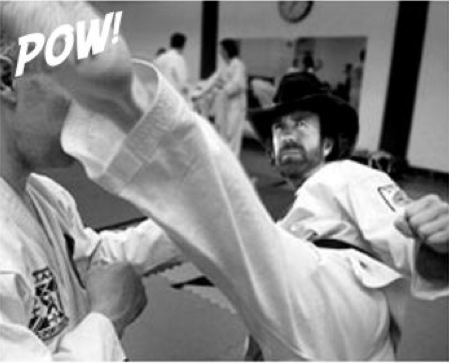
\includegraphics[scale=.8]{img/chuck.png}
    \caption{G2G Formation rocks}
    \label{norris}
\end{figure}
\end{verbatim}
\begin{figure}[h]
    \centering
    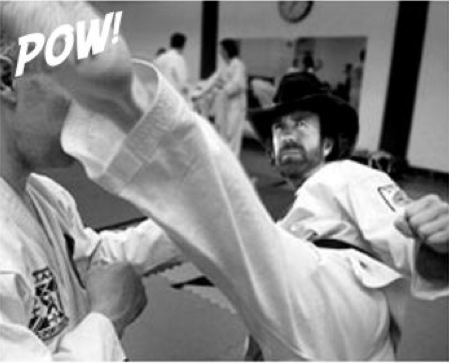
\includegraphics[scale=.7]{img/chuck.png}
    \caption{G2G Formation rocks}
    \label{img:norris}
\end{figure}
Per grafici e figure generate dall'utente si consiglia di utilizzare immagini di alta qualit\`a o meglio immagini vettoriali.
\begin{figure}[h]
    \centering
    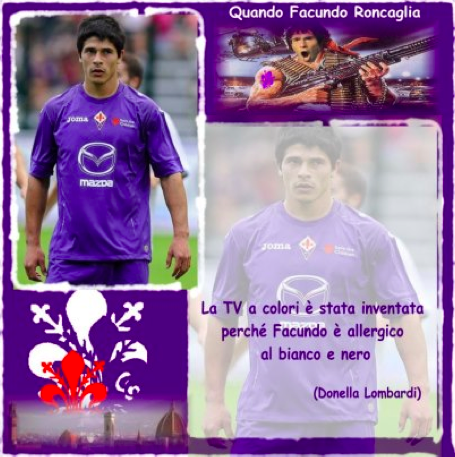
\includegraphics[scale=.7]{img/facundo.png}
    \caption{Quando Facundo}
    \label{img:facundo}
\end{figure}
Succede spesso infatti che una figura risulti ``sgranata'' e la divisione in pixel risulti evidente...proviamo con un'immagine pi\`u dettagliata (Figura \ref{img:facundo}).\\

 Dei pacchetti aggiuntivi quali PsTriks o Tikz, che generano l'immagine da un codice fornito dall'utente. Una valida alternativa per i principianti \`e l'editor latexdraw, un comodo tool scritto in java che permette di esportare il codice PsTricks o un'immagine in .pdf da un disegno eseguito dall'utente. La comodit\`a di questo editor sta nella possibilit\`a di inserire formule all'interno delle immagini.
\begin{figure}[h]
    \centering
    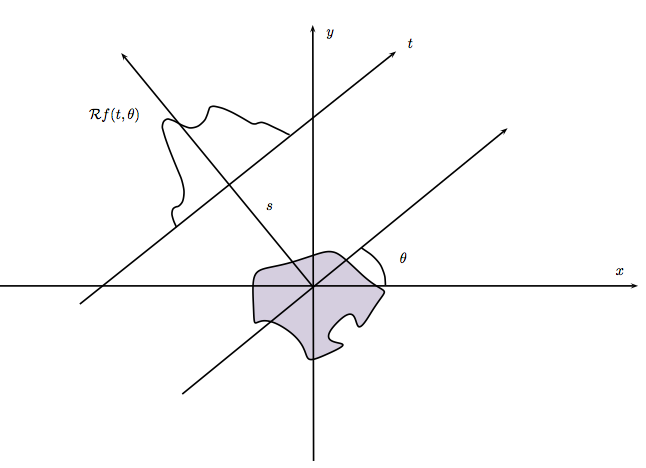
\includegraphics[scale=.9]{img/radon.png}
    \caption{Esempio di figura in latexdraw: la trasformata di Radon: $\mathcal{R} f (t,\theta) =\int_{\mathbb{R}} f (t\cos\theta-s\sin\theta , t\sin\theta + s\cos\theta) \, ds$}
    \label{ldraw}
\end{figure}
\\
\scatola{Ma cosa mi importa delle immagini vettoriali?}\\
Il \LaTeX{} \`e pensato in modo vettoriale, pensa al vantaggio di poter zoomare all'infinito una figura. La qualit\`a della pagina stampata poi \`e molto migliore rispetto all'immagine raster!
\subsection{Teoremi}
\textit{Theorem} \`e un ambiente utile per i matematici, ma personalizzabile, per chiunque voglia creare all'interno del testo un'area separata con la struttura del tipo:\\
\textbf{Titolo \# numerotitolo} \textit{Intestazione o spiegazioni, anche lunghe e dettagliate, che richiedono pi\`u di una riga}. In modo da rendere maggiormente visibile una parte importante del testo o un concetto fondamentale. Le definizioni vanno nel preambolo
\begin{verbatim}
\newtheorem{theorem}{Teorema}[section]
\end{verbatim}
Vediamo un esempio:
\begin{verbatim}
\begin{theorem}
Chi si loda si sbroda.
\end{theorem}
\begin{proof}
Chi parla troppo bene di se' stesso effettivamente pu\`o finire per
sovrastimare le proprie reali capacit\`a...certo che questo non dimostra
niente, non \`e vero in generale!
\end{proof}
\end{verbatim}
\begin{theorem}
Chi si loda si sbroda.
\end{theorem}
\begin{proof}
Chi parla troppo bene di se' stesso effettivamente pu\`o finire per
sovrastimare le proprie reali capacit\`a...certo che questo non dimostra
 niente, non \`e vero in generale! \textbf{Dimostrazione fallita!}
\end{proof}
Questo fa pensare alle differenze fra il pensiero comune e il pensiero matematico...
\subsection{Riferimenti incrociati}
\scatola{Ma a che servivano, scusa tutti quegli href? una formula magica??}\\
Dato che la gestione del posizionamento nel testo degli ambienti \textit{table} e \textit{figure} \`e decisa dal compilatore, spesso ci troviamo nel bisogno di fare riferimento a un'immagine, a un teorema, a un ambiente la cui posizione nel testo \`e lontana, magari in qualche capitolo precedente. Per far fronte al problema dei riferimenti abbiamo messo delle etichette o \textit{label} all'interno degli oggetti precedenti, che quindi richiamiamo quando ci fa comodo con il comando
\begin{verbatim}
\ref{nome}, \eqref{nome equaz}
\end{verbatim}
le equazioni possono anche essere chiamate con ref, ma eqref le indica come sono scritte, fra parentesi. Questo pu\`o sembrare una pignoleria, ma \`e di fatto pi\`u comodo a chi legge un testo scientifico avere chiaro da subito la natura del riferimento scritto in testo.\\
Per esempio possiamo parlare di quanto ci \`e utile l'equazione \eqref{equaz}, spiegata intuitivamente in Figura \ref{ldraw} \fbox{non \`e vero, che c'entra??} e come si pu\`o dedurre dalla Tabella \ref{tabella}.\vspace*{.5cm}\\
 \scatola{Si, poi? se uno mi deduce l'identit\`a di Euler da una tabellina pitagorica fatta male \`e davvero un mostro!!}\\
Ti ringrazio per lo spirito critico, ma era solo un esempio...\\
In conclusione i riferimenti possono alleviare le sofferenze di chi legge e di chi scrive...inoltre il pacchetto \textit{href} permette di linkare tutti i riferimenti...Non ci credi? [\ref{norris}]
\subsection{Bibliografia}
Uno dei modi pi\`u semplici per ottenere una bibliografia \`e l'utilizzo dell'ambiente \textit{thebibliography}. Se nel testo vogliamo evidenziare o discutere il contributo letterario di B.B. Cluster, in particolare la sua opera principale ``Lettere di Carta'', invece che scrivere il riferimento al momento, possiamo evitare di appesantire il testo usando il comando:\\
\begin{verbatim}
\cite{codicelibro}
\end{verbatim}
A un certo punto del testo inseriamo la bibliografia
\begin{verbatim}
\begin{thebibliography}{biblio}
\bibitem{codicelibro} B.B. Cluster, \emph{Lettere di Carta}, ed. Lasesta, 1997
\bibitem{codicelibro2}......................
\end{thebibliography}
\end{verbatim}
E riferirsi al testo con una semplice formula quale:\\
Come scritto in \cite{bb}, Cap 1 p.132,.. per dimostrare l'identit\`a di Euler \eqref{equaz} basta una tavola pitagorica scrausa e sbilenca mostrata in Tabella \ref{tabella}.
\section{Modulo 4}
\subsection{Beamer}
Un altro tipo di documento di largo utilizzo \`e \textbf{beamer}, usato per creare presentazioni. Un beamer \`e un semplice documento .tex con nel preambolo il comando
\begin{verbatim}
\documentclass{beamer}
\usetheme{ }\end{verbatim}
dove il comando \textit{usetheme} contiene la scelta del tema per l'output. Di temi ce ne sono a dozzine per la rete, nel nostro esempio useremo il tema di un dottorando padovano\footnote{che ovviamente ringraziamo!}, disponibile sulla sua pagina web \\ \href{http://www.math.unipd.it/~burattin/other/tema-latex-beamer-padova/}{http://www.math.unipd.it/$\sim$burattin/other/tema-latex-beamer-padova/}.\\
Come si pu\`o vedere nell'esempio un file di questo tipo \`e molto simile ad un normale file \LaTeX{} con qualche differenza. Ad esempio, spesso si rinuncia agli ambienti \textit{equation}, \textit{figure} e \textit{table} in quanto in una presentazione poco spesso si ha il bisogno di inserire riferimenti incrociati.\\
Il testo \`e sempre diviso in sezioni e sottosezioni, talvolta riportate in una barra superiore (dipende dal tema scelto). Ogni slide \`e contenuta nel proprio ambiente \textit{slide}, all'interno del quale si inseriscono i contenuti. Le parti pi\`u importanti possono apparire dentro dei  blocchi, generati dagli ambienti \textit{block}, \textit{alertblock}, \textit{exampleblock}, ad esempio teoremi o avvertenze o esempi.\\
Volendo si pu\`o inserire del testo nella slide progressivamente con il comando \textit{pause}.


\subsection{Utilizzo di pacchetti aggiuntivi}
L'estensione di \LaTeX{} pu\`o essere potenzialmente infinita, mediante pacchetti aggiuntivi. Il sito di riferimento ufficiale per tali pacchetti \`e \href{http://www.ctan.org/}{http://www.ctan.org/}. Per installare un pacchetto bisogna scompattarlo nella cartella di riferimento texmf/tex/latex, avendo privilegi da amministratore.\\
\scatola{Si, e il povero mortale che deve scrivere nel laboratorio informatico, deve stare a rompere agli amministratori per ogni pidocchioso pacchettino che voglio provare?} \\
Ok, modo alternativo! nella home ti crei la cartella apposita cos\`i
\begin{verbatim}
$ mkdir -p ~/texmf/tex/latex/
\end{verbatim}
dentro la quale scompatterai il pacchetto appena scaricato, poi aggiornerai il programma sull'esistenza di questa cartella utile con il comando
\begin{verbatim}
$ texhash ~/texmf
\end{verbatim}
In seguito basta seguire gli esempi, e con un po' di creativit\`a i pacchetti aggiuntivi possono aiutarti a generare simboli, testo con font e ambienti nuovi oppure tipi di documento per le pi\`u svariate esigenze.

\subsection{Come trovare o creare simboli}
\scatola{Ho in mente un simbolo un po' strano da usare, ma non lo trovo nei prontuari..}\\
Prova a disegnarlo su questo sito
\href{http://detexify.kirelabs.org/classify.html}{http://detexify.kirelabs.org/classify.html} \`e un tool interessante, ti indica anche il pacchetto da usare per avere quel simbolo. Se non lo trovi devi usare un po' di inventiva, come in questo esempio:
\begin{verbatim}
La notazione usata dagli egiziani per indicare $1/n$ era
$\accentset{\begin{sideways} () \end{sideways}}{n}$
\end{verbatim}
La notazione usata dagli egiziani per indicare $1/n$ era $\accentset{\begin{sideways} () \end{sideways}}{n}$.\\
L'alternativa meno allettante \`e quella di impararsi ad usare metafont\footnote{non sono cos\`i avanti, mi spiace!}...
\subsection{Idee per un futuro migliore}
Siamo arrivati alla fine del nostro percorso guidato nel mondo del \LaTeX{} e volevo inserire un paio di provocazioni per nerd e sviluppatori hardcore:
\begin{enumerate}
 \item servirebbe integrazione fra beamer e impress.js per un nuovo stile di presentazione, che fonda le features del latex con un'impostazione pi\`u moderna e che includa facilmente filmati e gif animate (vera spina nel fianco di beamer).
\item non farebbe male, di questi tempi, un programma che compili il sorgente latex in ebook mobi/epub in modo efficiente e automatico, magari usando mathml...in questo modo ogni utente potrebbe crearsi il proprio ebook direttamente del sorgente .tex!
\end{enumerate}



\begin{thebibliography}{biblio}
\bibitem{bb} B.B. Cluster, \emph{Lettere di Carta}, ed. Lasesta, 1997
\end{thebibliography}
\end{document}
